\documentclass[10pt]{article}
\usepackage{amsmath,textcomp,amssymb,geometry,graphicx,enumerate,tikz,algorithm,algpseudocode,pifont,upgreek}
\usetikzlibrary{calc}
\usetikzlibrary{datavisualization}
\usetikzlibrary{datavisualization.formats.functions}


\textheight=9in
\textwidth=7in
\topmargin=-.75in
\oddsidemargin=-0.25in
\evensidemargin=-0.25in

\usepackage{listings}
\lstnewenvironment{codeblock}
    {\lstset{language=Python,
      showspaces=false,
      showtabs=false,
      breaklines=true,
      mathescape=true,
      showstringspaces=false,
      breakatwhitespace=true,
      commentstyle=\textit,
      keywordstyle=\textbf,
      basicstyle=\ttfamily,
      escapechar=`,
      moredelim={**[is][{\color{RoyalBlue}}]{\^^M\\beginsol}{\^^M\\endsol}},
      moredelim={[is][{\color{RoyalBlue}}]{\^^M\\beginexp}{\^^M\\endexp}},
    }}
    {}

\newcommand{\bigo}{\mathcal{O}}


\begin{document}
\section*{04/04/2016}
\subsection*{Neurons}
\begin{itemize}
	\item CPUs: largely sequential, nanosecond gates, fragile if gate fails, superior for 234x718, local rules, perfect key-based memories.
	\item Brains: very parallel, millisecond neurons, fault-tolerant, superior for vision, speech, associative memory.
	\begin{center}
		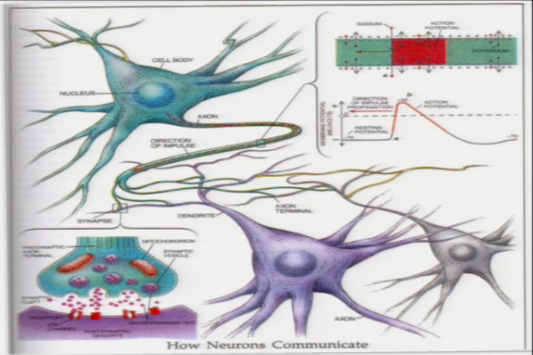
\includegraphics[scale=0.5]{../images/neurons}
	\end{center}
	\item \underline{Neuron}: a cell in brain/nervous system for thinking/communicating.
	\item \underline{Action potential} or \underline{spike}: An electrochemical impulse \underline{fired} by a neuro nto communicate with other neurons.
	\item \underline{Axon}: the limb(s) along which action potentials propagate; "output."
	\item \underline{Dendrite}: Smaller limbs by which neuron receives info; "input."
	\item \underline{Synapse}: Connection from one neuron's axon to another's dendrite.
	\item \underline{Neurotransmitter}: Chemicals released by axon terminal to stimulate dendrite.
	\item You have about $10^{11}$ neurons, each with about $10^{4}$ synapses.
	\item Analogies:
		\begin{itemize}
			\item Output of unit $\leftrightarrow$ firing rate of neuron.
			\item Weights of connection $\leftrightarrow$ synapse strength.
			\item Positive weight $\leftrightarrow$ excitatory neurotransmitters (e.g. glutamine).
			\item Negative weight $\leftrightarrow$ inhibitory neurotransmitters (e.g. GABA, glycibe)
			\item Linear combination of inputs $\leftrightarrow$ \underline{summation}.
			\item Logistic/sigmoid function $\leftrightarrow$ firing rate saturation.
			\item Weight change/learning $\leftrightarrow$ \underline{synaptic plasticity}. Hebb's rule (1949): "cells that fire together, wire together.""
			\begin{center}
				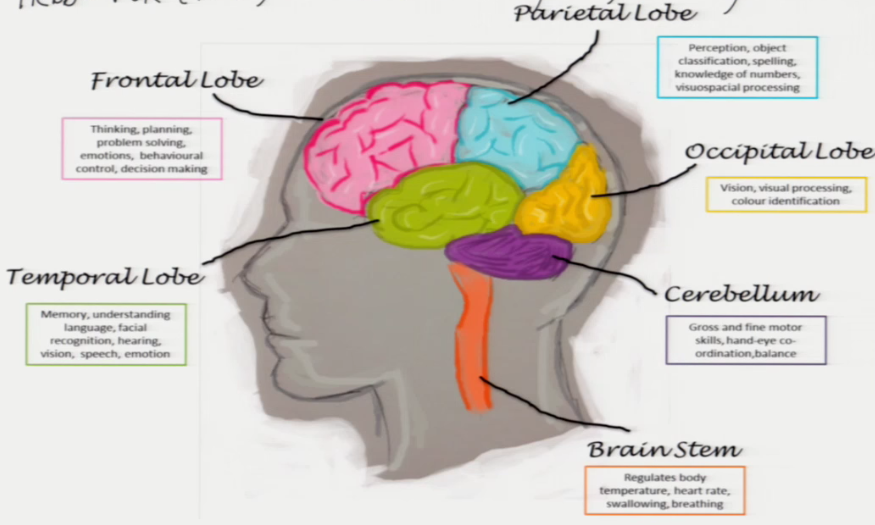
\includegraphics[scale=0.5]{../images/brain}
			\end{center}
		\end{itemize}	
\end{itemize}

\subsection*{Neural Net Variations}
\begin{itemize}
	\item Regression: Usually omit sigmoid function from output unit(s).
	\item Classification:
		\begin{itemize}
			\item Logistic loss function (aka \underline{cross-entropy}) often preferred to squared error:
			\begin{align*}
				L(z,y) = -\sum_{i} (y_{i}\ln z_{i} + (1-y_{i}) \ln (1-z_{i}))
			\end{align*}
			\item For 2 classes, use one sigmoid output; for $k \geq 3$ classes, use \underline{softmax} function.
				\begin{itemize}
					\item Let $t = Wh$ be $k-$vector of linear combination in final layer.
				\end{itemize}
		\end{itemize}
		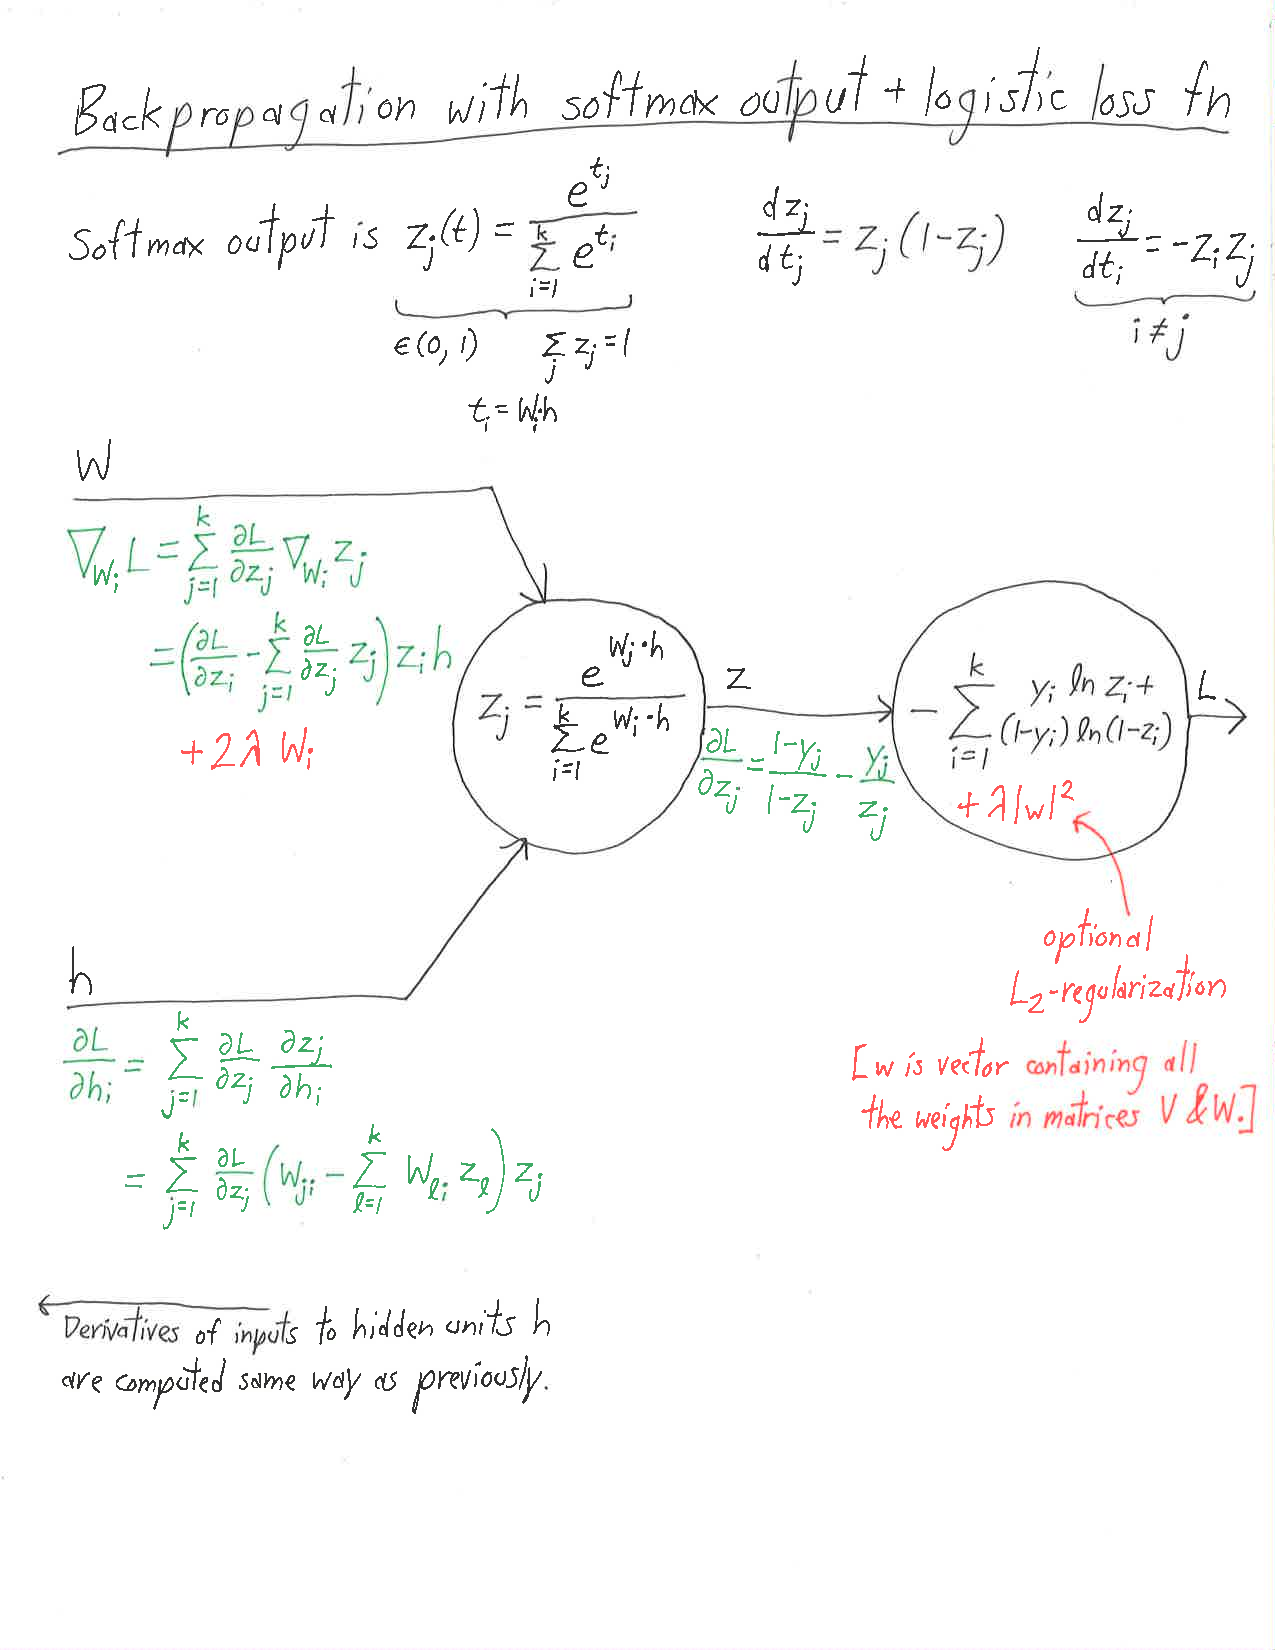
\includegraphics[scale=0.7]{softmaxprop}
	
	\newpage
	\subsubsection*{Unit Saturation}
	\begin{itemize}
		\item Problem: when unit output $s$ is close to 0 or 1 for all training points, $s' = s(1-1) \approx 0$, so gradient descent changes $s$ very slowly. Unit is "stuck." Slow training and bacd network.
		\begin{center}
			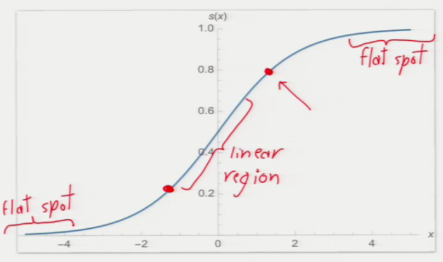
\includegraphics[scale=0.7]{../images/unitsaturation}
		\end{center}
		\item Mitigation: 
			\begin{enumerate}
				\item Set target value $(y)$ to 0.15 and 0.85 instead of 0 and 1.
				\item Modify back-propagation to add small constant (typically $\sim$ 0.1) to $s'$.
				\item Initial weight of edge into unit with fan-in $\upeta$: random with mean zero, standard deviation $\sqrt{\upeta}$.
				\item Replace sigmoid with ReLUs: \underline{rectified linear units}. \underline{ramp function} aka \underline{hinge function}:
				\begin{center}
					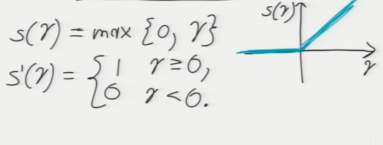
\includegraphics[scale=0.7]{../images/hinge}
				\end{center}
			\end{enumerate}
	\end{itemize}
	
	\subsubsection*{Heuristics for Avoiding Bad Local Minima}
	\begin{itemize}
		\item 1 or 4 above.
		\item Stochastic gradient descent. A local minimum for batch descent is not a minimum for one typical training point.
		\item Momentum. Gradient descent changed "velocity" slowly. Carries us right through shallow local minima to deeper ones.
\begin{codeblock}
	$\Delta w \leftarrow -\epsilon \nabla w$
	repeat:
	    $w \leftarrow w + \Delta w$ ($\Delta w$ is speed)
	    $\Delta w \leftarrow - \epsilon \nabla w + \beta \Delta w$ ($\beta$ how strongly momentum persists. $0 \leq \beta < 1$)
\end{codeblock}
	\end{itemize}
\end{itemize}

\end{document}